\documentclass[prb,twocolumn]{revtex4-1}
\usepackage{times}
\usepackage{bbm}
\usepackage[dvips]{graphicx}
\usepackage{latexsym,amsmath,amssymb,bm,euscript}
\usepackage[dvips]{color}
\usepackage{multirow}
\usepackage{calligra}

\DeclareMathAlphabet{\mathcalligra}{T1}{calligra}{m}{n}
\DeclareFontShape{T1}{calligra}{m}{n}{<->s*[2.2]callig15}{}

\newcommand{\scripty}[1]{\ensuremath{\mathcalligra{#1}}}

\def\ra{\rangle} % bra
\def\la{\langle} % ket
\def\uz{U(1)\times\mathbb{Z}_2}
\def\ztwo{\mathbb{Z}_2}
\begin{document}

\title{}
\date{\today}
\pacs{}

\author{Scott D. Geraedts}
\author{Olexei I. Motrunich}
\affiliation{Department of Physics, California Institute of Technology, Pasadena, California 91125, USA}

%%%%%%%%%%%%%%%%%%%%%%%%%%%%%%%%%%%%%%%%%%%%%%%%%%%%%%%%%%%%%%%
\begin{abstract}
\end{abstract}
%%%%%%%%%%%%%%%%%%%%%%%%%%%%%%%%%%%%%%%%%%%%%%%%%%%%%%%%%%%%%%%
\maketitle

\section{Introduction}
%The study of topological phases of matter has been a major component of condensed matter research for the past several years. Among the many phases studied, the topological insulator (TI) is one of the most prominent. The TI is a three-dimensional phase of free fermions. Though it is insulating in the bulk, its topological behavior can be deduced from its unusual surface properties, in particular the odd number of Dirac cones it has on its surface. The topological insulator is an example of a symmetry-protected topological phase (SPT). Like all SPT's, it has short-ranged entanglement, which implies that is has a unique ground state on any closed manifold. This is in contrast to topologically ordered states like the fractional quantum Hall effect. The topological insulator has both charge conservation and time-reversal symmetry, and if either of these symmetries are broken it loses its topological properties.

%One obvious extension of research into topological insulators is to consider the effects of interactions on their properties. This is however a difficult task. Many of the methods used to study TI's involve the properties of their band structure, and these methods obviously do not apply to the interacting case. As an introduction to this difficult problem, one can try to study an analog of the topological insulator, constructed of interacting bosons instead of fermions. Certain theoretical techniques, like the Monte Carlo studies employed in this paper, work for only for bosonic systems. In addition, in bosonic systems we know that the non-interacting case would be a condensate, so we can sure that the topological behavior is due to the interactions.

%The study of topological phases of interacting bosons is relatively recent, but much progress has been made. Chen, Liu, Gu and Wen\cite{WenScience,*WenPRB} have used group cohomology theory to determine which symmetries and dimensions can lead to non-trivial topological phases. However, this approach tells us little about the properties of these phases, which must be determined through other methods. One well-studied case is that of SPT's in two dimensions with $U(1)$ symmetry. A Chern-Simons field theory has been found to describe both the bulk and edges of these systems.\cite{LuVishwanath} TIt can be shown that such systems have a Hall effect quantized to an even integer, (in units of $e^2/h$) and gapless edge modes. Therefore such systems are called `bosonic quantum Hall phases'. A powerful way to think about these phases is in the context of `flux-attachment', where we consider attaching a flux to each boson, in order to give the bosons non-trivial statistics.\cite{SenthilLevin} One drawback of the flux attachment technique is that it is not related to a microscopic model. To change this, in an earlier work we considered extending the symmetry to $U(1)\times U(1)$, i.e.~ two different species of bosons. Flux from one species of boson was bound to charge from the other species, and vice versa. In this way, we obtained a microscopic model which realized the bosonic quantum Hall effect, and studied this model in Monte Carlo.\cite{FQHE} 

%Interacting bosonic topological phases which are analogues of the topological insulator can also be considered. Senthil and Vishwanath\cite{SenthilVishwanath} have found effective field theories which can describe both the bulk and the surface of a three-dimensional topological phase with charge conservation and a $\mathbb{Z}_2$ symmetry. They find exotic behavior on the surface of their system which can be used to study the topological behavior in the bulk. The field theories can be constructed by adding an additional $SO(3)$ symmetry to the model, and binding monopoles of this symmetry to the bosons. Metliski and Fisher produced a construction which explicitly binds monopoles to bosons, and shown that it leads to the same topological phase. In that case the monopoles can be shown to come from the bosons themselves.\cite{Max} 

%In both the two- and three-dimensional cases, the topological behavior can be thought of as coming from the binding of bosons to point topological defects. In two dimensions the topological defects were vortices of another species of bosons, this was the flux attachment. In three dimensions the topological defects come from monopoles.

%In this work, we construct explicit models which realizes the interacting bosonic analog of the topological insulator. These models can be studied in Monte Carlo simulations. The main idea behind our constructions is the binding of monopoles to bosons, and condensation of the resulting bound states. We present two different models which realize this physics. In the first model, described in Section \ref{section::Heisenberg}, we introduce additional $SO(3)$ degrees of freedom in the form of Heisenberg spins. We can define `hedgehog' configurations from these spins, and these will serve as the topological defects which we bind to bosons. We introduce a term in our action which energetically binds hedgehogs to bosons, and we show that this term can lead to a phase (which we call the `binding phase') which is a condensate of these bound states.

%Our next task is to show that the binding phase is indeed topological. In the two-dimensional case, one can demonstrate topological behavior by measuring a bulk response which is topologically invariant: the Hall conductivity. In the three-dimensional case, no such response is known to exist. The most commonly cited evidence for topological behavior in the free fermion TI is the existence of an odd number of Dirac cones on the surface, but this diagnostic does not apply to our interacting case. Topological properties are often deduced by studying exotic physics on the surfaces of topological phases, and so we study the surface of the binding phase in Monte Carlo. We can determine the phase diagram of the surface and some of the properties of the surface phases, but we find no smoking gun that would indicate topological behavior. 

%The topological insulator, whether constructed from free fermions or interacting bosons, is believed to have a topological term in its effective field theory which leads to a quantized magneto-electric effect. This effect can possibly by introducing external electromagnetic gauge fields, and studying how they interact with the system.
%One measurement of this type which would indicate topological behavior is the Witten effect, in which magnetic monopoles of an external gauge field become bound to half a quanta of electric charge. Another measurement is the Hall effect at the surface of the topological phase. This bulk topological field theory becomes a Chern-Simons theory at the surface of the system, which, when time-reversal is broken at the surface, should lead to a Hall effect quantized in units of one-half the value allowed in a purely two dimensional system. In the bosonic quantum Hall effect the Hall conductivity is quantized to be an even integer, so if the binding phase is topological it should have a Hall conductivity on its surface with odd-integer values.

%In order to measure the above properties, we need to introduce external electromagnetic fields into our system. In the model in Section \ref{section::Heisenberg}, this is complicated by our definition of hedgehog number. In the main text, we will see that hedgehog number is a discontinuous function of the Heisenberg spins. When the external fields are introduced, the action becomes a discontinuous function of these fields, which prevents us from using linear response theory to measure the surface Hall conductivity. The form of the action after the external fields are introduced is also complicated, which makes it difficult to determine a configuration of external gauge fields which would correspond to the magnetic monopole needed to measure the Witten effect.To solve these problems, in Section \ref{section::CP1} we introduce a second model which binds monopoles to bosons. In this model, the additional $SO(3)$ degrees of freedom are described by CP$^1$ model instead of a Heisenberg model. The advantage of this formulation is that the action with the external gauge fields included has a relatively simple form. In particular, it is a continuous function of the external gauge fields, so linear responses such as the Hall conductivity can be computed.
%We determine the phase diagram of both the bulk and the surface of the new model. In the bulk, we introduce magnetic monopoles of the external electromagnetic field and measure one-half of a charge bound to them, precisely the predicted Witten effect. On the surface, we break the $\mathbb{Z}_2$ symmetry and find a Hall conductivity quantized to the predicted odd-integer values. 

%In Monte Carlo studies of the `bosonic quantum Hall' phases, we found additional topological physics by binding multiple topological defects to multiple bosons. In Section \ref{section::multiple} we consider such a binding of multiple bosons or multiple monopoles. In the case of multiple bosons, we find that phases made up of bound states containing an even number of bosons are topologically trivial, while if the bound states contain an odd number of bosons the system is in the topological phase. When bound states contain multiple monopoles, we find that the system is in a topologically ordered phase.

%%%%%%%%%%%%%%%%%%%%%%%%%%%%%%%%%%%%%%%%%%%%%%%%%%%%%%%%%%%%%%%%%%%%%%%%%%%%%%%%%%%%%%%%%%%%%%%5
\section{$SO(3)$ spins as a Heisenberg model}
\label{section::Heisenberg}

We first study the binding between topological defects and bosons by using hedgehogs of a Heisenberg model as our topological defects. We demonstrate the existence of a phase which is a condensate of bound states of hegehogs and bosons, and explore its properties. This model provides an intuitive introduction to the physics of binding defects to bosons, though we are unable to find conclusive evidence that the phase is topological.

\subsection{Bulk Phase Diagram}
\label{subsec::bulkheis}
We study the following action, in (3+1)-D Euclidean space-time:
\begin{equation}
S=S_{\rm spin}+\sum_{r,\mu} \frac{\lambda}{2}[ J_\mu(r)- Q_\mu(r)]^2.
\label{action}
\end{equation}
$S_{\rm spin}$ is an action which penalizes fluctuations in the $SO(3)$ spins. The second term describes the binding between bosons and hedgehogs. The bosons, $J_\mu$, are represented by integer-valued conserved currents defined on the links of a four-dimensional cubic lattice, where $r$ is the position on the lattice and $\mu\in (x,y,z,\tau)$ is a direction. These currents represent the world-lines of the bosons in the (3+1) dimensional space-time. The $Q_\mu$ variables represent the hedgehogs, which are also integer-valued conserved currents.  When the real number $\lambda$ is large, this term will bind bosons and hedgehogs together. We work with periodic boundary conditions, in the case with no net charge and no net hedgehog number, so that the $J_\mu$ and $Q_\mu$ currents have winding number zero.

We first represent the $SO(3)$ spins as unit vectors. This can be achieved with the following action, which describes a Heisenberg model:
\begin{equation}
S_{\rm spin}=-\beta\sum_{R,\mu} \vec{n}(R)\cdot \vec{n}(R+\mu).
\end{equation}
Here $\vec{n}$ are unit vectors which represent the spins. They exist on a different lattice from the $J_\mu$ and $Q_\mu$ variables above. This lattice has its sites labelled by $R$, and they are located at the centers of the (hyper)cubes of the lattice in Eq.~(\ref{action}). 
%more details about this?

From these unit vectors, we can define the hedgehog current $Q_\mu$ using the prescription in Ref.~\onlinecite{LesikAshvin,SachdevHedgehogs}, modified to four dimensions. We summarize this prescription here. One first defines variables $\alpha_\mu(R)$, which exist on links connecting the spins $\vec{n}_i\equiv\vec n(R)$ and $\vec{n}_j\equiv\vec n(R+\mu)$:
\begin{equation}
e^{-i\alpha_{\mu}(R)}=\frac{1+\vec{n}_i\cdot\vec{n}_j+\vec{n}_i\cdot\vec{N}_0+\vec{n}_j\cdot\vec{N}_0+i\vec{N}_0 \cdot(\vec{n}_i\times\vec{n}_j)}{\sqrt{(1+\vec{n}_i\cdot\vec{n}_j)(1+\vec{n}_i\cdot\vec{N}_0)(1+\vec{n}_j\cdot\vec{N}_0})}.
\label{alpha}
\end{equation}
Here $\vec{N}_0$ is a reference vector which we choose arbitrarily. 
We then define placket variables $\omega_{\mu\nu}$ as follows:
\begin{equation}
\omega_{\mu\nu}(R)={\rm floor}[\alpha_\mu(R+\nu)-\alpha_\mu(R)-\alpha_\nu(R+\mu)+\alpha_\nu(R)].
\label{omega}
\end{equation}
One can show that changing the reference vectors $\vec{N}_0$ changes each $\alpha$ variable by a phase, and these phases cancel in the definition of $\omega_{\mu\nu}$ so that it is independent of the reference vector. Finally, we can define the hedgehog current:
\begin{equation}
Q_\mu(r)=\frac{1}{2}\epsilon_{\mu\nu\rho\sigma}\nabla_{\nu} \omega_{\rho\sigma}(R).
\label{monopoledef}
\end{equation}
If we consider only three dimensions of our four-dimensional lattice, the $\omega_{\mu\nu}$ involved in the definition of $Q_\mu$ make up a cube on the lattice indexed by $R$. We have defined the lattices so that there is a vertex of the lattice labelled by $r$ at the center of this cube, and this is where the $Q_\mu$ variables are defined. When all four dimensions are considered, this vertex becomes a link in the $\mu$ direction.  

The above action can be studied in Monte Carlo. In addition to simple updates of $\vec{n}$ and $J_\mu$, when $\lambda$ is large one needs to try updates which change both $J_\mu$ and $Q_\mu$ in such a way that the second term in Eq.~(\ref{action}) is unchanged. To do this we choose a spin and an amount to update it, and check to see if any $Q_\mu$ variables will change as a result of this update. If so we attempt to update $J_\mu$ and $n$ simultaneously.

In this work, we monitor the ``internal energy per site'', $\epsilon= S /{\rm Vol}$, where ${\rm Vol}\equiv L^4$ is the volume of the system, which has linear size $L$. From this, we can determine the specific heat:
\begin{equation}
C=(\la \epsilon^2\ra-\la\epsilon\ra^2)\times{\rm Vol}.
\end{equation}
We can locate phase transitions in our model by looking for singularities in the specific heat. We also monitor the magnetization per spin of the $SO(3)$ spins:
\begin{equation}
m=\la |\sum_R \vec{n}(R)|\ra/{\rm Vol}.
\end{equation}
When the spins are disordered, the average of the magnetization is proportional to $1/\sqrt{\rm Vol}$. Therefore we can use measurements of magnetization at different sizes to determine if the spins are ordered.

To study the behavior of the boson currents, we monitor current-current correlators, defined as:
\begin{equation}
\rho_J({k})=\la J_\mu({k})J_\mu(-{k})\ra
\end{equation}
where $k$ is a wave vector and 
\begin{equation}
J_\mu({k})\equiv\frac{1}{\rm \sqrt{Vol}}\sum_r J_\mu(r)e^{i{k}\cdot r}.
\end{equation}
In the bulk of the system, $\rho_J({k})$ is independent of the direction $\mu$, and when we show numerical data we average over all directions to improve statistics. We evaluate the correlators at the smallest non-zero ${k}$, i.e.~if $\mu$ is in the $x$ direction, we average over ${k}_{min}=(0,\frac{2\pi}{L},0,0)$, $(0,0,\frac{2\pi}{L},0)$, and $(0,0,0,\frac{2\pi}{L})$. We also monitor the current-current correlators of the hedgehog currents, $\rho_Q(k)$, which are defined in the same way as for the boson currents.

In the phase where the $J_\mu$ are gapped, $\rho_J\sim {k}_{\rm min}^2$, while when the $J_\mu$ proliferate $\rho_J$ is independent of system size. Therefore we can use finite-size scaling of this quantity to determine the locations of phase transitions. For the hedgehog currents, $\rho_Q\sim {k}_{\rm min}^2$, everywhere, so we cannot use finite-size scaling of these variables to find phase transitions. 

To determine the phase diagram of the bulk of this model, it is convenient to define new variables
\begin{equation}
\tilde J_\mu(r)=J_\mu(r)-Q_\mu(r).
\label{shift}
\end{equation}
Expressed in these variables, the first and second terms in Eq.~(\ref{action}) decouple, and we can study them independently. 
At small $\beta$, the $\vec{n}$ spins are disordered, which also implies that the hedgehog currents are proliferated. As $\beta$ is increased, the spins order. This means that there is a large energy cost for hedgehog currents to exist. We say that the hedgehog currents are gapped, and only small loops of them are allowed. We can determine the location of the spin-ordering phase transition by finding singularities in the heat capacity, or by performing finite-size scaling on the magnetization as described above. The value found by our numerics agrees with the literature.\cite{McKenzie2}

At small $\lambda$, the $\tilde J_\mu$ variables are proliferated. In our original variables, this means that the boson currents are independent of the hedgehog currents. At large $\lambda$, the $\tilde J_\mu$ variables are gapped. The boson currents are bound to the hedgehog currents. The results of this can be seen in Fig.~\ref{heisbulk}, which shows the current-current correlators for the boson and hedgehog currents. Initially there is no correlation between the bosons (red line) and the hedgehogs (blue line). As $\lambda$ is increased, the current-current correlators become identical as the bosons and hedgehogs are bound together. We can determine the location of the phase transition in $\lambda$ by studying singularities in the heat capacity, or by peforming finite-size scaling on $\rho_{\tilde J}$ as described above. The inset in Fig.~\ref{heisbulk} shows the phase diagram. At small $\lambda$ and $\beta$, both the boson and hedgehog currents proliferate and are not bound. At small $\lambda$ and large $\beta$ hedgehog currents are gapped, but boson currents proliferate, while at large $\lambda$ and $\beta$ all currents are gapped. When $\lambda$ is large and $\beta$ is small the system is in the `binding' phase, which we will argue is a topological phase.

\begin{figure}
\includegraphics[angle=-90,width=0.9\linewidth]{figures/heisbulkout.eps}
\caption{Inset: Phase diagram for the bulk of the Heisenberg version of the model. The phase diagram is equivalent to a system of decoupled currents and spins. At $\lambda=0$, the system has a paramagnet-ferromagnet transition as $\beta$ is increased. As $\lambda$ is increased, the boson currents bind to the hedgehog currents. The loops in the phases show a `snapshot' of the phase. Red loops mean that boson currents are proliferated in the phase, while blue loops indicate proliferated hedgehog currents. The phase of interest is the upper left is the `binding' phase where bosons are bound to hedgehogs. The main figure shows the current-current correlations of the bosons and hedgehogs as $\lambda$ is increased while $\beta=0$. We see that the correlators become equal as the system enters the upper left phase, indicating that bosons have bound to hedgehogs.}
\label{heisbulk}
\end{figure}

In this work we will make use of a $\ztwo$ symmetry of our action, which is obtained by reflecting the $\vec{n}$ spins around a plane. To see how this affects the hedgehog current, we can examine Eq.~(\ref{alpha}), taking the reference vector $N_0$ to be in the plane of reflection. We see that reflecting the spin changes only the complex part of $e^{i\alpha_\mu}$, and therefore the hedgehog current changes sign under such a reflection. For our entire action to have this reflection symmetry, we therefore need to combine such reflections with a ``charge-conjugation'' operation which takes changes the sign of the boson charge. For concreteness we label the directions the $\vec n$ spins can point in as $(a,b,c)$, and we will consider the $\ztwo$ symmetry corresponding to reflections in the $ab$ axis. In this case the $\ztwo$ symmetry can be summarized as:
\begin{equation}
\begin{array}{ccc}
n_a,n_b & \rightarrow & n_a,n_b \\
n_c & \rightarrow & -n_c\\
Q_\mu & \rightarrow & -Q_\mu\\
J_\mu & \rightarrow & -J_\mu 
\end{array}
\end{equation}.

It is also helpful to think in terms of the `easy-plane' picture of the $SO(3)$ spins, in which the spins are roughly in the $ab$-plane, with only small $c$ components. In the easy-plane picture we can define `vortices' of the $U(1)$ spins which are the $ab$-components of the $\vec n$ variables. 
The vortices are defined on the plackets of the cubic lattice. Therefore in the Monte Carlo they are represented as two-dimensional `world-sheets'. When dealing with vortices, one can gain intuition by thinking in terms of only the three spatial dimensions of our (3+1) dimensional space-time. In this picture the bosons and hedgehogs are represented by point particles, while the vortices are represented by lines. The results of the next several paragraphs can be most easily understood by thinking in this picture.

%It is instructive to consider various subgroups of the $SO(3)$ symmetry. First, we can get a $\mathbb{Z}_2$ subgroup by considering reflecting the $\vec{n}$ spins around any plane. To see how this affects the hedgehog current, we can examine Eq.~(\ref{alpha}), taking the reference vector $N_0$ to be orthogonal to the direction of reflection. We see that reflecting the spin changes only the complex part, and therefore $Q_\mu\rightarrow-Q_\mu$ under such a reflection. For our entire action of have this reflection symmetry, we therefore need to combine such reflections with a ``charge-conjugation'' operation which takes $J_\mu\rightarrow -J_\mu$. 

%We label the three directions the $\vec n$ spins can point in as $(a,b,c)$. In this work, we find it convenient to consider a $U(1)\times \mathbb{Z}_2$ subgroup of the $SO(3)$ symmetry. Here the $\mathbb{Z}_2$ symmetry is a reflection around a plane described as above, which for concreteness we take to be the $ab$-plane. The $U(1)$ symmetry is a rotation in the $ab$-plane.  We can then think of our spins in an ``easy-plane'' picture where the spins are roughly in the $ab$-plane, with only small $c$-components. Though this picture of course breaks the $SO(3)$ symmetry, the $U(1)\times \mathbb{Z}_2$ symmetry is unbroken. In the easy-plane picture we can define `vortices' of the $U(1)$ spins which are the $ab$-components of the $\vec n$ variables. 

Though ordinary $U(1)$ spins are not defined at the core of a vortex, our spins have a $c$-component which can point either up or down at the vortex core. We can define two species of vortices, which we call the $\uparrow$ and $\downarrow$ species, depending on whether $n_c$ is positive or negative. This description is useful since an $\uparrow$ vortex on top of a $\downarrow$ vortex is a hedgehog. Therefore our system can be thought of as a system of vortex lines of two different species. These vortex lines can change species, and the locations where they change species are hedgehogs. This picture is shown in Fig.~\ref{monopoles}.

Hedgehog number can have either positive or negative values, and this is determined by the properties of the vortex line they are attached to. 
We can determine these relations by considering the behavior of our model under reflections in the $ab$ and $ac$ planes. 
Reflection around the $ab$-plane (as described above) interchanges $\uparrow$ and $\downarrow$ vortex lines, while reflection around the $ac$-plane changes the vorticity of the vortex lines, from clockwise to counter-clockwise and vice-versa. Both of these operations change the charges of the hedgehogs and bosons.
Let us define a positive hedgehog charge to be one which turns an $\uparrow$ vortex into a $\downarrow$ vortex, on a clockwise vortex line (pictured third from left in Fig.~\ref{monopoles}). The charges of other hedgehogs can be determined from the above symmetries, and are shown in Fig.~\ref{monopoles}. 

\begin{figure}
\includegraphics[angle=-90,width=0.95\linewidth]{figures/monopoles.eps}
\caption{As discussed in the text, our system has two species of vortex lines, $\uparrow$ and $\downarrow$. A hedgehog is a transition point between the two types of lines, with the charge of the hedgehog determined by the orientation of the vortex lines and their vorticity. Applying a Zeeman field to the surface means allowing only one type of vortex line through the surface. This leads to a correlation between the hedgehog charge and the vorticity at the surface, which is the origin of the Hall conductivity. This figure shows only the spatial dimensions of the system, therefore the hedgehogs are point particles and the vortices are lines.}
\label{monopoles}
\end{figure}

We are claiming that the phase where hedgehogs proliferate and are bound to bosons is a symmetry-protected topological phase, which is protected by both the $U(1)$ symmetry from the conserved boson charges, and the $SO(3)$ symmetry from the spins. Therefore breaking either of these symmetries should destroy the phase. Breaking the boson charge symmetry allows the total boson charge in the system to fluctuate and so to have binding we need also need to allow fluctuations in the hedgehog number. The periodic boundary conditions in our system force the total hedgehog number to always be zero. Therefore we cannot simulataneously have binding between bosons and hedgehogs and a fluctuating total boson charge, and so breaking this $U(1)$ symmetry destroys the binding phase.

We can break the $SO(3)$ symmetry by introducing a Zeeman field into our action:
\begin{equation}
S_{\rm Zeeman}=\sum_R h n_c(R).
\label{Zeeman}
\end{equation}
Here $h$ is the strength of the Zeeman field, which points in the $c$-direction. In our picture of two species of vortices (Fig.~\ref{monopoles}), the Zeeman field forbids one of the species. Since the vortex lines cannot change species, hedgehogs are forbidden and the binding phase is destroyed. 

%%%%%%%%%%%%%%%%%%%%%%%%%%%%%%%%%%%%%%%%%%%%%%%%%%%%%%%%%%%%%%%%%5
\subsection{Surface Phase Diagram}
\label{subsec:heissurf}
By analogy to the fermionic topological insulator, we expect that one way to investigate the topological nature of our phase is to study the physics of its surface. 
We introduce a surface between the binding phase and the trivial insulator by using the spatially varying function $\eta(r)$ so that Eq.~(\ref{action}) becomes:
\begin{equation}
S=S_{\rm spin}+\sum_r \frac{\lambda}{2}[J_\mu(r)-\eta(r) Q_\mu(r)]^2.
\end{equation}
We vary $\eta(r)$ in the $z$ direction, so that:
\begin{equation}
\eta(r)=
\left\{ \begin{array}{cc}
1 & z_L\leq z<z_R\\
0 & \rm{otherwise}\\
\end{array}\right..
\end{equation}
This leads to the binding phase between $z_L$ and $z_R$, while the trivial phase occupies the rest of the space. Note that there are two surfaces of the SPT region: one at $z_L$ and one at $z_R$.

On the surface, we can measure all of the quantities which we measured in the bulk, but we now only sum over the sites near the surface, and when averaging over all directions we only use the $x$, $y$ and $\tau$ directions. 

The binding between hedgehogs and bosons in the bulk of the topological phase leads to exotic physics on the surface. In both the binding and trivial phase, hedgehog currents proliferate, while boson currents are bound to the hedgehog currents in the binding phase but are absent in the trivial phase, as shown in Fig.~\ref{surface}. Consider what happens when a hedgehog loop tries to cross the boundary between the phases. The boson current has to form a closed loop, and it can do this by running along the edge. This implies that we have an unbound boson, which incurs a high energy cost. Despite this high energy cost, this situation may occur in our system. Another possibility is that hedgehogs will be forbidden from crossing the surface.

\begin{figure}
\includegraphics[angle=-90,width=0.9\linewidth]{figures/surface.eps}
\caption{A snapshot of the system, when it is spatially divided into a region which is a trivial insulator and a region which is in the binding phase. In the trivial phase boson currents are gapped and hedgehog currents proliferate. In the binding phase both currents are gapped individually, and they must form bound states. Large hedgehog current loops can exist in either region, but when such a loop tries to cross the boundary it leaves boson currents on the surface. Pictured is the case where hedgehogs currents cross the surface and lead to bosons condensing on the surface. Alternatively hedgehog currents could be energetically forbidden from crossing the boundary.}
\label{surface}
\end{figure}

One way to show that our system is topological is to find physics on the surface of the binding phase which cannot exist in a purely (2+1) dimensional bosonic system. 
Such physics is not guaranteed to exist, for example we may find that the surface of the system is a phase which breaks all the symmetries of the system. This phase could exist on the surface of either a topological or trivial phase, and therefore does not provide evidence that our system is topological. Alternatively, though we may suspect that exotic physics exists on the surface phase, we may not know of a way to detect it in Monte Carlo. 
%For example, some exotic surface phases thought to exist are identified by fractional charge or statistics in their gapped excitations, which we do not know how to detect. 

Despite these obstacles, a good place to start looking for topological behavior of the binding phase is to identify the phases on the surface. To do this, we fix the values of $\beta$ and $\lambda$ in the bulk and tune them only on the surface, by setting:
\begin{equation}
\beta,\lambda=\left\{
\begin{array}{cc}
\beta_{\rm surf},\lambda_{\rm surf} & z=z_R,~\mu=\hat{x},\hat{y},\hat{z}\\
\beta_{\rm bulk},\lambda_{\rm bulk} & {\rm otherwise }
\end{array}\right.
\label{bulkvsurf}
\end{equation}
We obtain the phase diagram in the inset of Fig.~\ref{heissurf}, which contains three distinct phases. When $\lambda_{\rm surf}$ is small the bosons are in a superfluid phase, breaking their $U(1)$ symmetry. This is the scenario pictured in Fig.~\ref{surface}, where monopoles can cross the surface, and these crossings are connected by boson currents. If $\beta_{\rm surf}$ is also small the $SO(3)$ symmetry is unbroken as the spins are disordered. As $\beta_{\rm surf}$ increases the $SO(3)$ symmetry breaks. At large $\lambda_{\rm surf}$ bosons see a large energy cost, and so the $U(1)$ symmetry is unbroken. This forbids hedgehogs from crossing the surface, leading to a system of $SO(3)$ spins with hedgehogs forbidden, which is known to break the $SO(3)$ symmetry.\cite{LauDasgupta} All data was taken with $\beta_{\rm bulk}=0$, $\lambda_{\rm bulk}=5.2$, parameters which put the bulk deep into the binding phase.

If there is behavior in any of the above surface phases which would confirm that the binding phase is topological, we do not know how to identify it in Monte Carlo. We must therefore look beyond this phase diagram. However, there is one promising feature of the phase diagram, which is a direct transition between the $U(1)$ unbroken, $SO(3)$ broken phase and the $U(1)$ broken, $SO(3)$ unbroken phase. This is unusual since one would naively expect that, without fine-tuning, the $U(1)$ and $SO(3)$ symmetry-breaking transitions would occur in different places. Though this does not definitively show that the binding phase is topological, it does provide evidence that we have an unusual field theory on the surface. 

Figure~\ref{cp1surfphase} shows evidence that we do in fact have a direct transition. We have plotted magnetization and $\rho_J$ on the surface, with $\beta_{\rm surf}=0$ and various $\lambda_{\rm surf}$. The $SO(3)$ symmetry is broken when $M\sqrt{\rm Vol}$ grows with system size, and the boson charge $U(1)$ symmetry is broken when $\rho_J$ starts to increase. We can see that everywhere one of the symmetries is broken, and we also see only one peak in the heat capacity on such a sweep. These results imply that we have a direct transition between the two phases.

%For example, if we tune $\beta$ and $\lambda$ so that the bulk of the system is in the binding phase, and study the surface, we find that the $SO(3)$ symmetry has spontaneously broken on the surface. This corresponds to the case where hedgehogs are forbidden from crossing the boundary. We know that the surface of a topological phase can spontaneously break symmetry, but a trivial phase can as well, and therefore this does not provide evidence that the binding phase is topological. We can try to find a more exotic phase by tuning $\beta$ and $\lambda$ only on the surface. We expect that at small $\lambda$  bosons on the surface condense, leading to a spontaneously broken $U(1)$ symmetry. There may also be an intermediate phase where hedgehogs crossing the surface are only partially suppressed, leading to a more exotic phase.\cite{LesikAshvin} 
%The phase diagram of the surface of the binding phase is shown in the inset of Fig.~\ref{heissurf}. We see three distinct phases, which break either the $U(1)$ symmetry of the bosons, the $SO(3)$ symmetry of the spins, or both symmetries. We see no phases without a broken symmetry. Therefore this phase diagram not tell us whether the binding phase is topologically non-trivial. The phase diagram was determined by studying singularities in specific heat, as well as the magnetization, and boson current-current correlators. Fig.~\ref{heissurf} shows an example of the data used to determine the phase transitions. We have plotted magnetization and $\rho_J$ on the surface, with $\beta_{\rm surf}=0$ and various $\lambda_{\rm surf}$. The $SO(3)$ symmetry is broken when $M\sqrt{\rm Vol}$ grows with system size, and the boson charge $U(1)$ symmetry is broken when $\rho_J$ starts to increase. We can see that everywhere one of the symmetries is broken, so there is no intermediate phase. We also see only one peak in the heat capacity on such a sweep, implying the existence of only one phase transition.

\begin{figure}
\includegraphics[angle=-90,width=0.9\linewidth]{figures/heissurf.eps}
\caption{The inset shows the phase diagram of the surface of the Heisenberg version of the model, without a Zeeman field. It was obtained by tuning the bulk into the phase where bosons and hedgehogs are bound, and then tuning $\beta$ and $\lambda$ {\em only on the surface}.  We find that our surface always spontaneously breaks  a symmetry. At small $\beta$ and $\lambda$ the $U(1)$ symmetry breaks and the bosons condense into a superfluid, while at large $\lambda$ the $SO(3)$ symmetry breaks and the spins align into a ferromagnet. At small $\lambda$ and large $\beta$ both symmetries are broken. Symmetry breaking on the surface is consistent with the bulk being topological, but is also consistent with the bulk being topologically trivial. The main plot shows magnetization and boson current-current correlators, on a sweep in $\lambda_{\rm surf}$ for $\beta_{\rm surf}=0$. The magnetization is rescaled so that it is constant in system size in the disordered phase, and grows with system size in the ordered phase. The current-current correlators start to increase when the bosons condense. We see that there is a direct transition between the two phases. All data in this section was taken with bulk parameters $\beta=0$, $\lambda=5.2$.}
\label{heissurf}
\end{figure}

Another possible way to observe exotic physics on the surface is to apply a Zeeman field to it, with the hope of seeing an unusual Hall conductivity. By analogy with the fermionic case, if we observe a Hall conductivity quantized to one-half of the smallest possible two-dimensional value, it is evidence that our system is in a topological phase. We apply a Zeeman field by adding a term similar to Eq.~(\ref{Zeeman}) to our action, but only on the surface of the model. Also, the fields $h$ on the two surfaces have opposite signs.

Hall conductivity in this system of bosons and vortices will be due to correlations between vorticity of the spins and the boson charges,\cite{FQHE} so we will measure these correlations directly before moving on to the more complicated Hall conductivity measurement. In the absence of the Zeeman field, we can use the symmetry of reflection of the $\vec n$ variables in the $ab$-plane to change the sign of the boson charge without changing the vorticity, and so such correlations vanish. This can be seen in Fig.~\ref{monopoles}, where, for example, on the top surface there is one clockwise vortex attached to a positively charged hedgehog (which is in turn bound to a positively charged boson), and another clockwise vortex is attached to a negatively charged hedgehog. Applying a Zeeman field corresponds to only allowing one type of vortex line to pass through the surface. In Fig.~\ref{monopoles}, this means that only solid lines are allowed to pass through the top surface. We can see that this leads to a correlation between the vorticity of the vortex on the surface and the charge of the hedgehog it is attached to. 

To measure correlations between vortices and bosons we first compute vorticity $V_{\mu\nu}(r)$ using the following formula:
\begin{eqnarray}
&&V_{\mu\nu}(r)=s_{\mu}(R)-s_{\mu}(R-\nu)-s_{\nu}(R)+s_{\nu}(R-\mu)\\
&&s_{\mu}(R)\equiv \left[\arctan\left(\frac{n_a(R)}{n_b(R)}\right) -\arctan\left(\frac{n_a(R-\mu)}{n_b(R-\mu)}\right)\right]{\rm mod}~2\pi.\nonumber
\end{eqnarray}
The vorticity is defined on the plackets of the $R$ lattice, however in four dimensions a placket on the $R$ lattice is also a placket on the $r$ lattice, so we can define the vorticity on the same lattice as the bosons. We can then Fourier transform the vorticity as follows:
\begin{equation}
V_{xy}(k)=\frac{1}{\sqrt{L^3}}\sum_{r}  ^\prime V_{xy}(r) e^{ik\cdot r}.
\end{equation}
The prime on the sum indicates we have summed over all sites at a fixed $z$, which is chosen to be at the surface. We can then measure $\la V_{xy}(k_{\rm min})J_\tau(k_{\rm min})\ra$, and the results are shown in Fig.~\ref{heishall}. 

We see that as soon as a Zeeman field is applied, the vortices and charges become correlated. Unlike the Hall conductivity, we do not expect these correlations to approach any universal value. We do note that the correlations on the two surfaces of the model are approximately equal, which is encouraging as we would expect the Hall conductivity on these surfaces to be equal as well.

In order to measure Hall conductivity, we need to couple both the bosons and spins to external probing fields, and then use linear response theory to determine the conductivity. When we do this we run into a problem, which has to do with the way the hedgehog currents $Q_\mu$ were defined. We can see from Eq.~(\ref{omega}) that in the definition of $Q_\mu$ we employed the discontinuous function floor$(x)$. When including the probing fields, this causes the path integral to the a discontinuous function of the probing fields, which prevents us from using linear response theory, and so we do not know how to calculate conductivity in this system. In the next section we will discover a way around this problem.

\begin{figure}
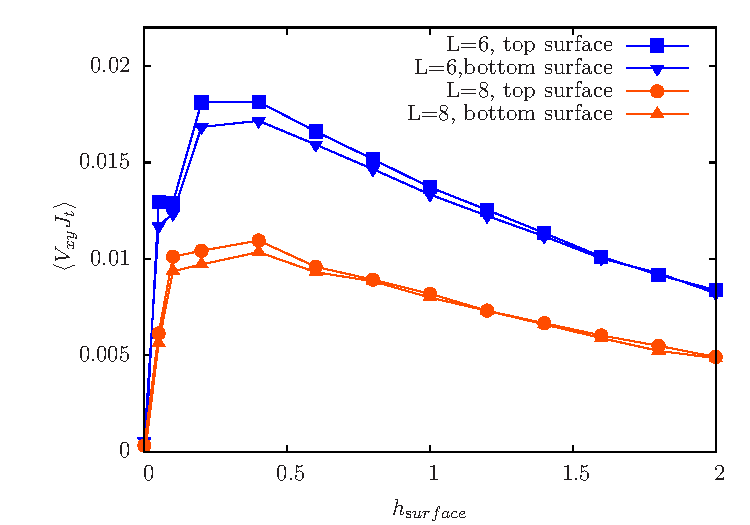
\includegraphics[angle=-90,width=0.9\linewidth]{figures/vortexcor.eps}
\caption{Charge-vortex correlators near the surface for the Heisenberg version of the model. The $x$-axis is the strength of the Zeeman field, applied only near the surface. We see that as soon as a Zeeman field is turned on, the correlator takes a non-zero value. The value is non-universal, but is approximately the same on the top and bottom surfaces. Since we do not know how to use linear response theory on this system we are unable to compute the Hall conductivity. Data was taken with $\beta=0$, $\lambda=5.2$.}
\label{heishall}
\end{figure}



%%%%%%%%%%%%%%%%%%%%%%%%%%%%%%%%%%%%%%%%%%%%%%%%%%%%%%%%%%%%%%%%%%%%%%%%%%%%%%%%%%%%%%%%%%%%%%%5

\section{$SO(3)$ spins using $CP^1$ representation}
\label{section::CP1}

In order to overcome some of the shortcomings of representing the $SO(3)$ spins as a Heisenberg model, we now describe these variables using a CP$^1$ theory. 
This theory has spinor matter fields (``spinons'') coupled to a compact gauge field and is a faithful representation of the microscopic spin system with short-range interactions, i.e., such a lattice ``field theory'' is ``emergable'' from a local microscopic Hamiltonian. We will see that this allows us to measure the Hall conductivity on the surface. It will also allow us to see other exotic surface physics, as well as a Witten effect in the bulk.

\subsection{Bulk Phase Diagram}
The following action represents the $SO(3)$ spins in the $CP^1$ representation:
\begin{eqnarray}
&&S_{\rm spin}=-\beta\sum_{s=1,2}\sum_{R,\mu} [z_s^\dagger(R)z_s(R+\hat\mu)e^{-ia_\mu(R)}+c.c.] \nonumber\\
&&+K\sum_{R,\mu<\nu} \cos[\nabla_\mu a_\nu(R)-\nabla_\nu a_\mu(R)].
\label{cp1action}
\end{eqnarray} 
In this representation the $SO(3)$ spins are represented by two complex bosonic fields $z_1$,$z_2$. We can write the $z$ fields as a spinor, $\mathbf{z}\equiv(z_1~z_2)^T$, and this allows us to extract the $SO(3)$ spin $\vec{n}=\mathbf{z^\dagger} \vec\sigma \mathbf{z}$, where $\vec{\sigma}\equiv (\sigma_a,\sigma_b,\sigma_c)$ is a vector of Pauli matrices, with the indices $a,b,c$ used instead of the familiar $x,y,z$ to avoid confusion with the lattice direction indices.
%The spin, $\vec{n}$, can be extracted from the $z$ fields by writing them as a spinor , 
The bosonic fields are minimally coupled to a compact gauge field $\vec{a}$. The last term is similar to a Maxwell term for the compact gauge field. The variables in the above action live on a cubic lattice, where position on the lattice is given by $R$ and $\mu$,$\nu$ are directions.

We find it convenient to break the $SO(3)$ symmetry down to $U(1)$ explicitly by taking the ``easy-plane'' limit of the $CP^1$ model. This means that we align all the spins $\vec{n}$ in the $ab$-plane. This corresponds to fixing the magnitude of $z_1$ and $z_2$, and allowing only phase fluctuations, i.e. $z_s\equiv \frac{1}{\sqrt{2}}e^{i\phi_s}$ The $CP^1$ model in the easy-plane limit becomes:
\begin{eqnarray}
&&S_{\rm spin}=-\beta\sum_{s=1,2}\sum_{R,\mu} \cos[\nabla_\mu\phi_s(R)-a_\mu(R)]\nonumber\\
&&+\sum_{R,\mu<\nu}\frac{K}{2}\left[\nabla_\mu a_\nu(R)-\nabla_\nu a_\mu(R)-2\pi B_{\mu\nu}(R)\right]^2.
\label{sspin}
\end{eqnarray}
Here $\phi_1$ and $\phi_2$ are $2\pi$-periodic variables which represent the phases of the boson fields. We have also rewritten the last term in a ``Villain'' form where the cosine is replaced by the above term, with $B_{\mu\nu}$ an unconstrained, integer-valued dynamical variable which lives on the plackets of the lattice. Upon summing over all $B_{\mu\nu}$, the third term is still a $2\pi$ periodic function of $a_{\mu}$, and therefore this does not change the universality class of the problem.

Using the Villain form in the third term is advantageous as it allows us to define the hedgehog current:
\begin{equation}
Q_\mu(r)=\frac{1}{2}\epsilon_{\mu\nu\rho\sigma}\nabla_\nu B_{\rho\sigma}(R).
\label{mondef}
\end{equation}
Note that $Q_\mu(r)$ resides on the links of the lattice labelled by $r$ which, as in the previous section, is interpenetrating with the lattice labelled by $R$. This gives the $B_{\mu\nu}$ variables the meaning of Dirac strings of the hedgehogs.

In what follows it is often convenient to think in terms of the `parton' description of Matlitski and Fisher \cite{Max}. In this description, the CP$^1$ model arises from thinking about splitting a boson into two 'partons', which carry opposite charges equivalent to one-half of the boson charge. More explicitly, in this description a boson creation operator is equivalent to the product of a creation operator of one parton and an annihilation operator of the other. Splitting a boson into partons in this way introduces an internal gauge field, whose charge is carried by both partons. In Eq.~(\ref{sspin}), $\phi_1$ and $\phi_2$ can be thought of as the phases of the different species of partons, and $a_\mu$ is the internal gauge field. 

The model described by  Eqs.~(\ref{action}) and (\ref{sspin}) can be studied in Monte Carlo. Equilibration becomes difficult in the regime where $K$ and $\lambda$ are large, and it is necessary to include composite which simultaneously change multiple variables. One such update is to change $B_{\mu\nu}$ while also changing $J_\mu$ so that there is no change in the second term in Eq.~(\ref{action}). Another update is to change both $a_\mu$ and $B_{\mu\nu}$ in such a way as to minimize the second term in Eq.~(\ref{sspin}). We also need to do an update which changes $a_\mu, B_{\mu\nu}$ and $J_\mu$. 

In the easy-plane model we have explicitly broken the $SO(3)$ symmetry, though we still have a $U(1)$ symmetry which corresponds to rotations in the easy-plane. The total symmetry of our system is now $U(1)\times U(1)\times\ztwo$. One of the $U(1)$ symmetries comes from the spin degrees of freedom, and the other comes from the bosons. The $\ztwo$ symmetry is the same as that in the previous section, 
 in the variables of Eq.~(\ref{sspin}) it can be summarized as
\begin{eqnarray}
&& \phi_1\rightarrow -\phi_2 \nonumber\\
&& \phi_2\rightarrow -\phi_1 \label{z2}\\
&& J_\mu \rightarrow -J_\mu \nonumber.
\end{eqnarray}

We can find the phase transitions in this model by looking for singularities in the specific heat, which is defined in the same way as the previous section. Order in the bosonic degrees of freedom can by identified by studying superfluid stiffness, while order in the spin degrees of freedom can by identified from the magnetization. In this easy-plane $CP^1$ version of the model, the spin degree of freedom is a $U(1)$ vector with components $n_x$, $n_y$. 
Its magnetization is given by:
\begin{equation}
m=\langle|\sum_R \exp[i\phi_1(R)-i\phi_2(R)]|\rangle /{\rm Vol} 
\end{equation}

The phase diagram in this model is parameterized by $\beta$, $K$ and $\lambda$. As in the previous section, we can make the change of variables in Eq.~(\ref{shift}) and find that the boson part of the problem decouples from the $CP^1$ part. The phase diagram of the boson part is the same as in the previous section. When $\lambda$ is small, the bosons are independent of the hedgehogs. As $\lambda$ is increased, they become bound to hedgehogs. The transition happens at $\lambda\approx 4$. 
The location of the phase transitions in the spin degrees of freedom are independent of $\lambda$, though the nature of the various phases are not. In Fig.~\ref{cp1bulkphase} we show at phase diagram in the $\beta$ and $K$ variables, for two cases: $\lambda$ small and $\lambda$ large. The locations of the phase transitions are consistent with the easy-plane CP$^1$ model in the literature.\cite{LesikSenthil} 
Let us first consider the case when $\lambda$ is small. When $\beta$ and $K$ are both small, the spin degrees of freedom are disordered and the hedgehogs can proliferate. The phase is therefore a trivial paramagnet in the spin degrees of freedom, and a superfluid in the boson degrees of freedom. 
As $K$ is increased, hedgehogs acquire a large energy cost, and become gapped. This phase has been studied in Ref.~\onlinecite{LesikSenthil}. It is known as the Coulomb phase because it has an emergent photon, and gapped excitations that carry charge $1/2$ and interact via a Coulomb interaction. This phase is also a superfluid in the boson degrees of freedom. 
The phase at large $\beta$ and $K$ has a large energy penalty for spin fluctuations, and so the spins order. This phase is a trivial ferromagnet in the spin degrees of freedom and a superfluid in the boson degrees of freedom. In the case when $\lambda$ is large, the spin parts of the Coulomb and ferromagnetic phases do not change. However in these phases are now trivial insulators in the boson degrees of freedom. However, in the paramagnetic phase the bosons become bound to hedgehogs of the spins. This is the binding phase, which we will argue is a topological phase.
 
%The phase diagram of the spin degrees of freedom is shown in Fig.~\ref{cp1bulkphase}, and is consistent with the literature on the easy-plane $CP^1$ model.\cite{LesikSenthil} The locations of the phase transitions are independent of $\lambda$, but the nature of the phases can depend on whether $\lambda$ is large or small. In Fig.
%In the phase at small $\beta$ and large $K$, monopoles are gapped but the $\phi$ variables can fluctuate. 
%This phase has been studied in Ref.~\onlinecite{LesikSenthil}. It is known as the Fractionalized Coulomb phase because it has an emergent photon, and gapped excitations that carry charge $1/2$ and interact via a Coulomb interaction. At large $\beta$ the spins are ordered. In both of these phases, monopoles are gapped. Therefore the bosons are independent of the spin degrees of freedom, and the transition as $\lambda$ is increased causes these bosons to become gapped. 
%At small $\beta$ and $K$, the spin degrees of freedom are disordered, and monopoles can proliferate. This phase is a trivial insulator. At small $\lambda$, the bosons are condensed but independent of the spins, while at large $\lambda$ the bosons are now bound to the monopoles, which are proliferated.  

%The phase diagram in this model is parameterized by $\beta$, $K$ and $\lambda$. In Fig.~\ref{cp1bulkphase}, the phase diagram is shown as a function of $\beta$ and $K$. As in the previous section, we make the change of variables in Eq.~(\ref{shift}) and find that the boson part of the problem decouples from the $CP^1$ part. Therefore the phase boundaries in Fig.~\ref{cp1bulkphase} are independent of $\lambda$. When $\lambda$ is small, there are three phases. At small $\beta$ and $K$, the spins are disordered and monopoles proliferate. This phase is a trivial insulator. At small $\beta$ and large $K$, monopoles are forbidden and the spins are disordered. This phase has been studied in Ref.~\onlinecite{LesikSenthil}, it has an emergent photon and its gapped excitations carry charge $1/2$ and interact via a Coulomb interaction. We call this the Fractionalized Coulomb phase. Finally, at large $\beta$ the spins are ordered. This model has been studied in Ref.~\onlinecite{LesikSenthil} and our phase diagram matches the one found in that work.
%In all of these phases, the bosons $J$ are condensed and independent of the rest of the system.

%We obtain a topological phase in our system by increasing $\lambda$, leading to a phase transition into a phase with binding between bosons and monopoles. As expected, the location of this phase transition is independent of $\beta$ and $K$. If the system at small $\lambda$ is in the Coulomb or magnetically-ordered phase, there are no monopole currents in the system. Therefore the $\lambda$ term simply gaps out the bosons, similar to the large $\beta$ case in Fig.~\ref{heisbulk}. If the system is in the trivial insulator, then increasing $\lambda$ will lead to the binding between bosons and monopoles that we believe will lead to a topological phase.

\begin{figure}
\includegraphics[angle=-90,width=0.9\linewidth]{figures/cp1bulkphase.eps}
\caption{Bulk phase diagram for the CP$^1$ version of the model, in the $\beta$ and $K$ variables. The top panel shows the phases at small $\lambda$, while the bottom panel shows large $\lambda$. The locations of the phase boundaries are independent of $\lambda$, but the nature of the phases is different. The candidate for the topological phase is the binding phase, which occurs at small $\beta$, small $K$ and large $\lambda$. Symbols indicate points where the phase transitions were identified numerically from singularities in the heat capacity.}
\label{cp1bulkphase}
\end{figure}

%%%%%%%%%%%%%%%%%%%%%%%%%%%%%%%%%%%%%%%%%%%%%%%%%%%%%%5
\subsection{Witten effect measurement}
In order to justify our claim that the binding phase is topological, we now demonstrate that our system exhibits a Witten effect. In a conventional free fermion topological insulator, the Witten effect is the phenomenon by which magnetic monopoles acquire a charge of one-half. In our system, we will introduce two external $U(1)$ gauge fields. One will couple to the spin degrees of freedom, and the other to the bosons. We will introduce a monopole in the spin external gauge field, and measure the total boson charge bound to it. Measuring a total charge quantized to one-half constitutes an observation of the Witten effect. 

The first step in measuring a Witten effect in our Monte Carlo is to add external gauge fields to the system. These external fields correspond to the `physical' charge of the system. We will fix configurations for these fields before performing the simulations, this corresponds to putting our system in some external electromagnetic field. These external gauge fields are distinct from the internal, dynamical gauge field $a_\mu$. Similarly, the external monopoles introduced in this section are different from the hedgehogs discussed previously, which are monopoles of the field $a_\mu$.
Let us first consider the gauge field coupled to the spin degrees of freedom. Here it is convenient to think in terms of the parton description in the previous section. Recall that in this description the spin degrees of freedom can also be thought of as coming from a boson. Here we will give this boson unit charge under an external compact gauge field we call $A_1$. The partons will carry charges $\pm 1/2$ under the field $A_1$, and unit charges under the field $a$. To modify Eq.~(\ref{sspin}) to reflect this, we add $\pm A_1/2$ inside the cosines on the first line. We should also include a Maxwell term for the external gauge field. As in Eq.~(\ref{sspin}), we use the `Villain' form of the Maxwell term, which introduces integer-valued placket variables $M_{\mu\nu}$. We can define external monopoles from these variables using the same techniques as in the previous section. Finally we also want to couple another external gauge field, which we call $A_2$, to the boson variables $J$. All of these changes combine to give us the following action. 
\begin{eqnarray}
&&S=-\beta\sum_{R,\mu} \cos[\nabla_\mu\phi_1(R)-a_\mu(R)+\frac{1}{2}A_{1\mu}(R)]\nonumber\\
&&-\beta\sum_{R,\mu} \cos[\nabla_\mu\phi_2(R)-a_\mu(R)-\frac{1}{2}A_{1\mu}(R)]\nonumber\\
&&+\sum_{R,\mu<\nu}\frac{K}{2}\left[\nabla_\mu a_\nu(R)-\nabla_\nu a_\mu(R)-2\pi B_{\mu\nu}(R)\right]^2\nonumber\\
&&+\sum_{R,\mu<\nu}\frac{K}{2}\left[\nabla_\mu A_{1\nu}(R)-\nabla_\nu A_{1\mu}(R)-2\pi M_{\mu\nu}(R)\right]^2.\nonumber\\
&&+\sum_{r,\mu} \frac{\lambda}{2}[ J_\mu(r)- Q_\mu(r)]^2+iJ_{\mu}(r)A_{2\mu}(r)
\label{withA}
\end{eqnarray}

The Villain variables $M_{\mu\nu}$ can be interpreted as the Dirac strings of the external monopoles. The Dirac strings of the external monopoles should be invisible to the partons, i.e. if a parton goes around a Dirac string, it should encircle a flux of $2\pi$. However, we also know that the partons carry only half a charge under the external gauge fields. Therefore naively the partons only see a $\pi$ flux from a Dirac string. The solution to this is for each Dirac string of the external monopoles to be bound to half of a Dirac string of the hedgehogs, $B_{\mu\nu}$. This will lead to a total $2\pi$ flux. We cause this to happen by enforcing the constraint that $2B_{\mu\nu}(R)=M_{\mu\nu}(R) (mod~2)$. 

We introduce an external monopole into our system by making a specific choice for the external variables $A_1$ and $M$. First, we choose a configuration of $M$ which will lead to a pair of monopoles. In our system of periodic boundary conditions, it is not possible to have only a single monopole. We will place external monopoles at coordinates $(x,y,z)=(0,0,0)$ and $(0,0,L/2)$, on the lattice labelled by $r$. The monopoles will have opposite charges, with the positively-charged one at the origin. All configurations of external gauge fields will be constant in the $\tau$ direction. In order to place external monopoles at these locations, we set $M_{xy}(R)=1$ whenever $x$ and $y$ are zero and $0\leq z<L/2$. All other $M_{\mu\nu}$ are set to zero. We must also constrain $B_{xy}$ to be odd half-integers on this Dirac string. Now that we have specified the $M$ values which introduce external monopoles, we choose values for the $A_1$ variables to minimize the action of the Maxwell term on the fourth line of Eq.~(\ref{withA}). In our simulations we will set $A_2=0$ everywhere, so that it does not affect the system. It will be used only when computing linear responses. 

There are in fact multiple configurations of the variables $M_{\mu\nu}$ which can lead to the same configurations of external monopoles. The physics of the system is independent of which configuration of $M_{\mu\nu}$ we choose because the various configurations are related by the following gauge transformation:
\begin{equation}
\begin{array}{ccc}
M_{\mu\nu}(R)&\rightarrow&M_{\mu\nu}(R)+\nabla_\mu \kappa_\nu(R) \\
B_{\mu\nu}(R)&\rightarrow&B_{\mu\nu}(R)+\frac{1}{2}\nabla_\mu \kappa_\nu(R) \\
A_{1\mu}(R)&\rightarrow&A_{1\mu}(R)+2\pi \kappa_\mu(R)\\
a_\mu(R)&\rightarrow&a_\mu(R)+\pi \kappa_\mu(R)
\end{array},
\end{equation}
where $\kappa_\mu(R)$ is an integer-valued field living on the links of the lattice labelled by $R$. One can use Eqs.~(\ref{mondef}) and (\ref{withA}) to check that this transformation does not change the monopole numbers or the action.

Having introduced external monopoles into our system, we can begin to see why they should carry half a charge of the boson gauge field $A_2$. 
The argument goes as follows. First, when modifying the Dirac string variables $M_{\mu\nu}$ to insert external monopoles, we were also forced to modify the variables $B_{\mu\nu}$ in such a way as to introduce one-half of hedgehog at the same location. However, we saw in the previous section that hedgehogs proliferate in the binding phase. Therefore the $1/2$-hedgehog which we introduced will be screened by a `cloud' of hedgehogs drawn from the rest of the system. This screening is analogous to Debye screening in a superconductor. The screening cloud will carry a hedgehog number of one-half, but with opposite sign to the first hedghog, leading to a total hedgehog number of zero. Since in the binding phase hedgehogs are bound to charges, the cloud also carries a boson charge of one-half. Therefore we find that half of a boson charge has bound to the external monopole.

%We can see this another way by recalling what happens to the action after applying the change of variables in Eq.~(\ref{shift}). The action becomes:
%\begin{equation}
%S=S_{\rm spin}+\sum_{r,\mu} \frac{\lambda}{2}\tilde{J}_\mu(r)^2.
%\label{actiontilde}
%\end{equation}
%In these variables the Dirac string introduces half of a hedgehog in the spin part of the action, and causes the $\tilde{J}$ variables to take only odd half-integer values. In the spin part, monpoles are condensed and so we cannot measure a monopole charge. The total $\tilde{J}$ charge will be $1/2~+$ an integer, and since the $\tilde{J}$ variables are gapped the integer will be zero and we measure a total charge of one half.

The above discussion is complicated by two degeneracies in Eq.~(\ref{withA}). The first is a degeneracy between $Q_\tau(0,0,0,\tau)=1/2$ and $Q_\tau(0,0,0,\tau)=-1/2$. In what follows it can be helpful to neglect the $\tau$ direction and think about $Q_\tau(0,0,0,\tau)$ as a stationary charge at the origin. Because of the degeneracy the statistical mechanics has each of the two states equally probable, which in an infinitely long simulation would lead to zero net internal monopole charge, and no Witten effect.
If we were able to fix the internal monopole current in one of these two states, for example $Q_\tau=1/2$, we have another degeneracy, between $J_\tau=0$ and $J_\tau=1$. This leads to a total boson charge of $1/2$ at the location of the external monopole. This charge cancels the boson charge from the screening cloud, leading to no Witten effect. 

Despite these degeneracies, we may still observe a Witten effect if the degenerate states are metastable, and the Monte Carlo is stuck in one of the two states. For example, in order to get from $Q_\tau=+1/2$ to $Q_\tau=-1/2$ one needs to modify all of the $\phi, a_\mu$ and $B_{\mu\nu}$ on the Dirac string, and such a move would be quite unlikely. Similarly, to get from $J_\tau=0$ to $J_\tau=1$ one needs to have a boson loop which runs from one external monopole to another, and such a step would have a high energy cost. 

On our finite systems, the system may be able to alternate between degenerate states. Initially, we find that the degeneracy in the $Q$ variables is unbroken, and we do not observe a Witten effect. We then break the degeneracy in the $Q$ variables by biasing the system with the following term:
\begin{equation}
\delta S_{\rm bias}=\gamma  \sum_{\tau}\left[J_\tau(0,0,0,\tau)-J_\tau(0,0,L/2,\tau)\right],
\label{bias}
\end{equation}
where $\gamma$ is some small real number. We have scanned the system by increasing $\gamma$ from zero and seen no divergence of correlation lengths, implying that these small $\gamma$ do not change the phase we are in. It would be surprising if the above biasing term affected the bulk physical properties of the system, as we are only making a modification to a fraction of the system proportional to $L^{-3}$. 

The effect of the biasing term is to break the degeneracy in the $Q$ variables, leading to $Q=+1/2$ at one external monopole and $Q=-1/2$ at the other. With or without the biasing term, in our Monte Carlo the system gets stuck in one of the $J$ states. Therefore we have broken the problematic degeneracies and removed the obstacle to measuring the Witten effect. We would like to stress that the Witten effect is ordinarily defined for a single monopole, in the thermodynamic limit. The problems we have with degeneracies are artifacts of the fact that we are trying to measure a Witten effect in a finite-size system with two monopoles. If Eq.~(\ref{withA}) were defined on an infinite system with only one external monopole, these problems would not arise.

Our measurements of the Witten effect will involve measuring the total charge enclosed in a sphere of radius $\scripty{r}$, centered around the location of the external monopole. Total charge is defined as:
\begin{equation}
{\rm charge}=\frac{1}{L}\sum_\tau \sum_{x^2+y^2+z^2\leq r} \langle J_\tau(x,y,z,\tau) \rangle.
\end{equation}
Simulations were perfomed with $L=10$, and the results are shown in Fig.~\ref{witten}.
At $\scripty{r}=0$, we are at the location of the monopole. There is no boson charge bound here. At $\scripty{r}=1$, we have already included most of the screening cloud, and therefore measure an enclosed charge close to $1/2$, as expected. The fact that $\scripty{r}=1$ measures a value close to one half shows that the screening length in the system is quite short. At $\scripty{r}=2$, we have included the entire screening cloud, so the charge is even closer to $1/2$. As $\scripty{r}$ is further increased, we start to include the screening cloud from the other external monopole, which is located at a distance $\scripty{r}=L/2$ from the first one. This cancels some of the charge from the first monopole, and so the total charge starts to decrease. When $\scripty{r}>L/2$, the sphere encompasses the screening clounds from both monopoles and so there is a net charge of zero. The values of charge are negative because we measured around a monopole of positive charge, and the sign of the charge in the screening cloud is the opposite of the sign of the external monopole. Note that the sphere discussed above is only a sphere in the $x$, $y$ and $z$ directions, and we have averaged over the $\tau$ direction.


\begin{figure}
\includegraphics[angle=-90,width=0.9\linewidth]{figures/wittenout.eps}
\caption{Measurement of the Witten effect. The inset shows the measurement setup. External monopoles, which carry internal monopole charge $\pm 1/2$, are inserted into the system, at a distance $L/2$ apart. They are Debye screened by internal monopoles of equal and opposite charge, which also carry half of a boson charge. The main plot shows the boson charge enclosed in a sphere of radius $\scripty{r}$. For small $\scripty{r}$, this sphere measures the boson charge in the screening cloud, and the result is $1/2$, as expected. For $r\approx L/2$ the sphere includes the charge from the other screening cloud, and since the charges are equal the enclosed charge drops to zero. The system size is $L=10$, using parameters $\beta=0.2$, $K=0.4$, $\lambda=8$, $\gamma=1.5$.}
\label{witten}
\end{figure}

In Fig.~\ref{witten}, we have found that the amount of charge at the site of the monopole ($\scripty{r}=0$), is zero. However, this is not universal and in fact depends on the choice of $\gamma$ in Eq.~(\ref{bias}). We could for example use a very large value of $\gamma$, which would introduce extra charge at $\scripty{r}=0$. However, the extra charge would not wind around the system $\tau$ direction, and so it would be compensated by less charge nearby. Therefore measurements taken far from the monopole would be unaffected. In our simulations, we find that $\scripty{r}=2$ is sufficiently far from the monopole to be unaffected by the change in $\gamma$. Figure~\ref{diffgamma} shows simulations taken with different values of $\gamma$. We see that though the amount of charge close to the monopole (near $r=0$ and $r=L/2$) can be affected by changing $\gamma$, the value at $\scripty{r}=2$ is always one-half, regardless of what $\gamma$ is used.
%We find that the screening cloud is very small, so that $r=1$ is sufficient to encompass the screening cloud and the sphere encloses half of a charge. As $r$ is increased, we still find half a charge enclosed. As $r$ is further increased, to $r=L/2-1$, the sphere starts to enclose charge from the screening cloud of the other, oppositely-charge external monopole, and this cancels some of the charge so that the enclosed charge starts to decrease. Finally, as $r$ is increased so as to enclose both screening clouds, the enclosed charge decreases to zero.

\begin{figure}
\includegraphics[angle=-90,width=0.9\linewidth]{figures/diffgamma.eps}
\caption{Witten effect for different values of $\gamma$, but all other parameters the same is in Fig.~\ref{witten}. We see that near $\scripty{r}=2$, when we are measuring the charge inside a sphere which surrounds exactly one external monopole, the amount of charge is approximately one-half, and independent of $\gamma$. At other values the enclosed charge does depend on $\gamma$.}
\label{diffgamma}
\end{figure}

Various other measurements can be made to support our conclusions. Measuring the total charge on each site shows that the half-charge is distributed around the external monopole in an approximately spherically symmetric way. Figure~\ref{wittenphase} shows the total charge on all the nearest-neighbours, as a function of $K$. We note that the Witten effect disappears at $K=0.6$, which is where the phase transition to the Coulomb phase is located. Compare this to Fig.~\ref{cp1bulkphase}.
%We can make Additionally, we have found that the bound charge is distributed isotropically around the external monopole. We can also detect the phase transitions in Fig.~\ref{cp1bulkphase} by measuring the Witten effect and observing that it vanishes outside the binding phase.


\begin{figure}
\includegraphics[angle=-90,width=0.9\linewidth]{figures/wittenphase.eps}
\caption{A demonstration of how the Witten effect can be used to detect phase transitions. The plot shows the amount of charge enclosed by a sphere with $\scripty{r}=2$, while changing $K$ but keeping all other parameters the same as in Fig.~\ref{witten}. We can compare to Fig.~\ref{cp1bulkphase}, and see that at $K=0.6$, when the system transitions from a topological phase to a trivial insulator, the Witten effect disappears.}
\label{wittenphase}
\end{figure}


%%%%%%%%%%%%%%%%%%%%%%%%%%%%%%%%%%%%%%%%%%%%%%%%%%%%%%%%%%%%%%%%%%55
\subsection{Surface Phase Diagram}

The measurement of the Witten effect is evidence that our binding phase is in fact topological. We can now study the exotic physics on the surface of this topological phase.

We define the surface as in Sec.~\ref{subsec:heissurf}. To uncover the exotic physics, we begin by performing a change of variables from the physical boson currents $J_\mu(R)$ to new integer-valued variables
\begin{equation}
G_\mu(r) \equiv J_\mu(r) - \eta(r) Q_\mu(r) ~,
\end{equation}
which satisfy 
\begin{eqnarray*}
\left(\sum_\mu \nabla_\mu G_\mu\right) (x, y, z, \tau) &=& 
\delta_{z, z_R} Q_z(x, y, z_R-1, \tau) \\
&-& \delta_{z, z_L} Q_z(x, y, z_R-1, \tau) ~. 
\end{eqnarray*}
The action for the spins and the new $G_\mu(r)$ variables is simply
\begin{equation}
S = S_{\rm spin} + \sum_{r,\mu} \frac{\lambda_\mu(r)}{2} \Big[G_\mu(r)\Big]^2 ~.
\end{equation}

For simplicity, from now on we consider situation where the trivial phase region and the SPT phase region are deep in their respective phases: in particular, $\lambda_{\rm bulk}$ (defined as in Eq.~(\ref{bulkvsurf} is very large.  At first we further simplify the situation by taking $\lambda_{\rm surf}$ to be very large, in which case we expect the variables $G_\mu(R)$ to be zero everywhere.  We also assume that $\beta$ is small everywhere, so the spin variables want to be deep in the disordered phase.  However, near the two surfaces, the spin configurations must satisfy
\begin{eqnarray}
Q_z(x, y, z_R-1, \tau) &=& 0, \\
Q_z(x, y, z_R-1, \tau) &=& 0.
\end{eqnarray}
Focusing on the spins near one surface, say at $z_R$, we can view $Q_z(x, y, z_R-1, \tau)$ as simply hedgehog numbers in the corresponding (2+1)-D spin system spanned by sites $(X, Y, Z=Z_R-1/2, T)$, and the above conditions correspond to complete suppression of hedgehogs in this spin system.  Such a (2+1)-D Heisenberg $O(3)$ spin model with hedgehog suppression was studied in Ref.~\onlinecite{LesikAshvin} and argued to be described by a \emph{non-compact} CP$^1$ field theory (NCCP$^1$).  On a simple (2+1)-D cubic lattice, such a model with complete hedgehog suppression actually has spontaneous magnetic order of spins even when the direct spin-spin interactions are zero.\cite{LauDasgupta, KamalMurthy}  However, more generic such models can have a spin-disordered phase with a propagating ``photon''\cite{KamalMurthy, LesikAshvin}, as well as other phases\cite{LesikAshvin2}.  Our findings in the present simulations on the surface of the SPT region are consistent with these earlier results.

Let us now proceed more systematically and, in particular, show how we obtain a generic NCCP$^1$ model on the surface of the SPT region.  For simplicity, we take $\lambda_{\rm bulk}$ to be very large. For finite $\lambda_{\rm surf}$, we need to keep $G_x, G_y, G_\tau$ degrees of freedom in the (2+1)D ``layer'' at $z_R$, while all other $G_\mu(r)$ are zero.  Focusing on the spin variables residing on sites $(x, y, z=z_R-1/2, \tau)$, the hedgehogs in this (2+1)D system are given precisely by $Q_z(x, y, z_R-1, \tau)$, which we will denote simply as $Q(x, y, \tau)$.  The structure of the surface theory is
\begin{eqnarray*}
S_{\rm surface} &=& S_{\rm matter-gauge} + \sum \frac{K}{2} ({\bm\nabla} \times {\bm a} - 2\pi {\bm B})^2 \\
&& + \sum \frac{\lambda_{\rm surface}}{2} {\bm G}^2 ~,
\end{eqnarray*}
subject to constraints
\begin{equation}
 \nabla_x G_x + \nabla_y G_y + \nabla_\tau G_\tau \equiv {\bm \nabla} \cdot {\bm G} = Q(x,y,\tau) \equiv {\bm \nabla} \cdot {\bm B} ~.
\end{equation}
Here $S_{\rm matter-gauge}$ represents the first term in Eq.~(\ref{cp1action}. The above is a 3D statistical mechanics model, $a_\mu$ and $B_{\mu\nu}$ from Eq.~(\ref{cp1action}) can be now defined as 3-vectors and are thus denoted by bold-face. 

This surface theory has spins plus integer-valued ``currents'' $G_\mu$ sourced and sinked by the hedgehogs of the spin system.  When the ``line tension'' $\lambda_{\rm surf}$ for the lines formed by these ``currents'' is large, we intuitively expect that the hedgehogs of the spin system are linearly confined.  It is not immediately clear, however, what happens when $\lambda_{\rm surf}$ is small.  Below we argue that the surface is still qualitatively described by the same ``hedgehog-suppressed'' field theory, which, however, can be in different regimes and have several different phases.

 We can deal with the constraints in the partition sum by changing to new variables
\begin{equation}
{\bm B}^\prime = {\bm B} - {\bm G} ~,
\end{equation}
which satisfy
\begin{equation}
{\bm \nabla} \cdot {\bm B}^\prime = 0 ~.
\end{equation}
The action becomes 
\begin{eqnarray*}
S_{\rm surface} &=& S_{\rm matter-gauge} + \sum \frac{K}{2} ({\bm\nabla} \times {\bm a}  - 2\pi {\bm B}^\prime - 2\pi {\bm G})^2 \\
&& + \sum \frac{\lambda_{\rm surface}}{2} {\bm G}^2 ~.
\end{eqnarray*}
There are now no constraints on the ${\bm G}$ variables, and we can formally sum these out to obtain some local action which is a function of ${\bm\nabla} \times {\bm a} - 2\pi {\bm B}^\prime$,
\begin{eqnarray*}
S_{\rm surface} &=& S_{\rm matter-gauge} + S_{\rm gauge, eff}[{\bm\nabla} \times {\bm a}  - 2\pi {\bm B}^\prime] ~.
\end{eqnarray*}
However, any such action with the compact variables ${\bm a}$ and divergenceless ${\bm B}^\prime$ can be formally viewed as describing a non-compact gauge field!  (In the limit of large $\lambda_{\rm surf}$, the effective action will have essentially lattice Maxwell form with stiffness $K$, while for intermediate to small $\lambda_{\rm surf}$ the gauge field energy will have more complicated but still local form.)  Thus, the field theory at the surface has the spinon matter fields coupled to a non-compact gauge field.  In particular, we expect that the surface can be in the same phases as the 3D NCCP$^1$ model.

%This exotic physics happens because, at large $\lambda$, the energy cost to have monopole loops cross the surface becomes very large, and we therefore cannot have monopoles on the surface. On the surface we then have a theory which is a CP$^1$ model with monopoles forbidden, also known as a {\em non-compact} CP$^1$ (NCCP$^1$) model. In this model, since monopoles are forbidden we have 
%\begin{equation}
%\epsilon^{\mu\nu\rho\sigma}\partial_{\nu}B_{\rho\sigma}=0,
%\end{equation}
%which means that $B$ can be written as:
%\begin{equation}
%B_{\mu\nu}=\nabla_\mu \alpha_\nu -\nabla_\nu \alpha_\mu,
%\end{equation}
%where $\alpha$ is some integer-valued variable living on the links of the lattice. We see that we can now write our action in terms of a non-compact internal gauge field:
%\begin{equation}
%\tilde{a}_\mu=a_\mu-2\pi\alpha_\mu.
%\end{equation}
%Therefore the effect of forbidding monopoles on the surface is to replace the compact field $a_\mu$ with the non-compact field $\tilde{a}_\mu$.

We can confirm the above arguments, which were made in some simplifying limits, by studying the system in Monte Carlo. We can determine the phase diagram of the surface by looking at singularities in the heat capacity. In this phase diagram we tune the bulk parameters so that the system is in the topological phase: specifically $\beta_{\rm bulk}=K_{\rm bulk}=0.2$, $\lambda_{\rm bulk}=8$. We then vary the surface parameters, and obtain the phase diagram shown in Fig.~\ref{cp1surfphase}, which is in good agreement with the phase diagram of the NCCP$^1$ model in the literature. Labels on the phase diagram are taken from Ref.~\onlinecite{LesikAshvin2}.
There are three phases in the diagram. At small $\beta_{\rm surf}$ the $\phi$ variables are disordered, conserving the spin $U(1)$ symmetry, while the boson $U(1)$ symmetry is broken. At large $\beta_{\rm surf}$, $K_{\rm surf}$ the spins order, leading to a Higgs phase which breaks the $U(1)$ symmetry from the spins but preserves the symmetry from the bosons. Finally at small $K_{\rm surf}$ and large $\beta_{\rm surf}$ both symmetries are broken. Here though the gauge field $a_\mu$ is free to fluctuate the spin degree of freedom, $\vec{n}$ is still ordered.

It is worth emphasizing here our point of view that the 3D NCCP$^1$ model with non-compact gauge field is not emergable as a theory for describing phases of a 2D local quantum Hamiltonian (the only exception is the deconfined quantum critical points that can render monopoles irrelevant dynamically). 

\begin{figure}
\includegraphics[angle=-90,width=0.9\linewidth]{figures/cp1surfphase.eps}
\caption{Surface phase diagram for the $CP^1$ version of the model. This diagram was obtained for $\beta_{\rm bulk}=0.2$, $K_{\rm bulk}=0.2$, $\lambda=8$, and parameters varied on the surface. The phase diagram has the same structure as the one found in the $NCCP^1$ model in Ref.~\cite{LesikAshvin2}. }
\label{cp1surfphase}
\end{figure}

It is also possible to have a topologically ordered phase on the surface\cite{SenthilVishwanath}. This can be accomplished by adding the following `pairing term' to the action:\cite{Max}
\begin{equation}
S_{\rm pair}=-t_{\rm pair}\sum_{R,\mu} \cos(\phi_1+\phi_2-2a_\mu).
\label{pairing}
\end{equation} 
We can now see what happens to the surface phase diagram (Fig.~\ref{cp1surfphase}) when $t_{\rm pair}$ is increased. For $t_{\rm pair}=2$, we get the phase diagram in Fig.~\ref{cp1surfpair}. We see that a new phase has opened up at small $\beta_{\rm surf}$ and large $K_{\rm surf}$. This phase does not break either of the $U(1)$ symmetries, and we believe it is a topologically ordered phase.


\begin{figure}
\includegraphics[angle=-90,width=0.9\linewidth]{figures/cp1surfacepairing.eps}
\caption{Surface phase diagram for the $CP^1$ version of the model, with the pairing term in Eq.~(\ref{pairing}). This diagram was obtained for $t=2$, $\beta_{\rm bulk}=0.2$, $K_{\rm bulk}=0.2$, $\lambda=8$, and $K_{\rm surf}$ and $\beta_{\rm surf}$ varied. Compared to Fig.~\ref{cp1surfphase}, we see that there is a new phase at large $K_{\rm surf}$ and small $\beta_{\rm surf}$. We expect that this surface phase is topologically ordered  }
\label{cp1surfpair}
\end{figure}

%%%%%%%%%%%%%%%%%%%%%%%%%%%%%%%%%%%%%%%%%%%%%%%%%%%%
\subsection{Surface Hall effect measurement}

In the free fermion topological insulator, it is predicted that one can apply a magnetic field on one surface of the system and measure on that surface a Hall conductivity quantized to $\frac{1}{2}\frac{e^2}{h}$. A similar effect is predicted in the case of the bosonic topological phase that we discuss.\cite{SenthilVishwanath} We can test this prediction in our simulations. The first step is to break the $\mathbb{Z}_2$ symmetry on the surface. By studying Eq.~(\ref{z2}), we see that the way to break the symmetry is to replace the parameter $\beta$ in Eq.~(\ref{sspin}) by the parameters $\beta_1$, which appears in the term containing $\phi_1$, and $\beta_2$, which appears in the term containing $\phi_2$. When $\beta_1-\beta_2\neq 0$, the $\mathbb{Z}_2$ symmetry is broken.

Consider the system with $K=0.4$ and $\lambda=8$ everywhere, $\beta=0.2$ in the bulk, and $\beta_{1}=\beta_{2}=0.2$ on the surface. This system will have its bulk in the topological phase, and its surface in the photon phase. We break the $\mathbb{Z}_2$ symmetry on one of the surfaces by increasing $\beta_{1}$. We expect that a small increase will not change the properties of the system very much, since both $\phi$ variables will still be in the photon phase.\cite{LesikAshvin2} However, as $\beta_1$ is further increased, vortices in the $\phi_1$ variables will become gapped. In our simulations we see a singularity in the specific heat, indicating that the system has entered a new phase. We expect that this phase will have a half-quantized Hall conductivity. In our simulations we also break time-reversal symmetry in the opposite direction on the other surface by increasing $\beta_2$. 

 We can see that unlike in the Heisenberg model, Eq.~(\ref{sspin}) is a differentiable function of the probing fields $A_1$ and $A_2$, and so we can use linear response theory to compute the Hall conductivity. We can apply the Kubo formula to Eq.~(\ref{withA}) as follows:
\begin{eqnarray}
&&\sigma_{\mu\nu}(k)=\lim_{A_1,A_2 \to 0}\frac{2\pi}{2\sin\left(\frac{\pi}{L}\right)}\frac{\partial^2 Z}{\partial A_{1\mu}\partial A_{2\nu}}~~~~~\\
&&=\frac{1}{2}\left\langle\xi_\mu(k)J_{\nu}(-k) \right\rangle,\nonumber
\end{eqnarray}
where
\begin{eqnarray}
&&\xi_\mu(k)=\sum_r \xi_\mu(r)e^{ikr}=\sum_R \xi_\mu(R)e^{ikR}e^{\frac{ik}{2}}\nonumber\\
&&\xi_\mu(R)\equiv\beta_1\sin(\nabla_u\phi_1-a_\mu)-\beta_2\sin(\nabla_\mu\phi_2-a_\mu)
\end{eqnarray}
$Z$ is the partition sum, and units are such that $e^2/h=1$. Note that care must be taken when Fourier transforming combinations of the $\phi$ and $a_\mu$ variables, since they reside on a different lattice than the $J_\mu$ variables. The measurements are performed at the smallest wave-vector $k$, as described in Section~(\ref{subsec::bulkheis}). Where we present numerical data we have averaged over the directions $\mu,\nu=x,y,\tau$. Note that the above conductivity measures the response of currents in gauge field $A_1$ to applied fields in gauge field $A_2$ (or vice-versa). In the literature these gauge fields are usually identified, which introduces an additional factor of two. In particular, when the gauge fields are identified the Hall conductivity of a two-dimensional system of bosons is quantized to $2$ times an integer (in units of $e^2/h$), while the Hall conductivity on the surface of a topological phase is an odd integer. Therefore where we present numerical values we have multiplied our results by $2$ so that they can be easily compared to the literature values.

We can gain some understanding of the origin of the Hall conductivity by considering the effect of a Zeeman field on Fig.~\ref{monopoles}. The Zeeman field forbids one type of vortex line from crossing the surface. We can see that when this is done, we introduce a correlation between the vorticity of the vortices on the surface, and the charge of the boson that they are bound to. Note that on one surface $\uparrow$ vortex lines are prohibited, while on the other $\downarrow$ lines are prohibited. We can imagine bringing the two surfaces closer together by shrinking the system in the $z$ direction. This will leave us with a quasi-two-dimensional slab on which vortices are bound to charges. We have studied such a system in a previous work,\cite{FQHE} and found that its Hall conductivity is quantized to be an even integer. It is reasonable to assume that this conductivity is evenly distributed between the two surfaces, leading to a half-integer conductivity on each surface. 

Figure \ref{cp1hall} shows our numerical measurements of the Hall conductivity. The $x$-axis is the strength of the Zeeman field. We see that initially there is no Hall conductivity, until the Zeeman field is strong enough to forbid one species of vortex. At this point the Hall conductivity increases until it reaches the value of approximately $1$. Though the value observed is actually slightly less than $1$, we believe that this is a finite-size effect, and indeed as system size is increased the Hall conductivity gets closer to the expected value. In addition to the plot shown, we have performed the same measurement for several different values of $K$, $\beta$ and $\lambda$, and found that the quantized result is independent of these parameters as long as we stay in the topological phase. This odd integer cannot be observed in a purely two-dimensional system, and therefore this observation shows that we are measuring the Hall conductivity on the surface of a topological phase.

\begin{figure}
\includegraphics[angle=-90,width=0.9\linewidth]{figures/cp1hall.eps}
\caption{Hall conductivity on the surface of the $CP^1$ version of the model, in units of $e^2/h$. On each surface we find that the conductivity is quantized to $1$, and this odd-integer value shows that we are on the surface of a topological phase. Data was taken for $K=0.4$, $\lambda=8$, $\beta_{\rm bulk}=0.2$. We measure the same conductivity on both the top and bottom surfaces of the topological phase.}
\label{cp1hall}
\end{figure}

%%%%%%%%%%%%%%%%%%%%%%%%%%%%%%%%%%%%%%%%%%%%%%%%%%%
\section{Binding of multiple bosons and hedgehogs}
\label{section::multiple}

In all of the above sections, we have studied a system where a single boson is bound to a single hedgehog. In this section we will describe the additional physics which arises when our system contains bound states of multiple bosons and/or multiple hedgehogs. We induce this multiple binding by making the following change to Eq.~(\ref{action}):
\begin{equation}
S=S_{\rm spin}+\sum_{r,\mu} \frac{\lambda}{2}[ dJ_\mu(r)- cQ_\mu(r)]^2.
\label{cdbind}
\end{equation}
Here $c$ and $d$ integers, and the action will bind $c$ bosons to $d$ hedgehogs. 

We first consider what happens when the bound states contain multiple bosons, which corresponds to $c>1$. In a similar system in two dimensions, we have found that each different $c$ leads to a different symmetry-protected topological phase.\cite{FQHE} In this case, however, the classification of Chen et al.\cite{WenScience,*WenPRB} predicts the existence of only one symmetry protected topological phase with this symmetry and in (3+1) dimensions. In agreement with this, we find that all systems with $c$ even are topologically trivial, while with $c$ odd we have the topological phase. 

We can justify this claim by showing that $c=2$ can be continuously connected to $c=0$ (which is a trivial insulator). This argument can then be extended to show that any two systems where $c$ differs by $2$ are in the same phase.
We start by considering two copies of our action, in the Heisenberg model and with $c=1$:
\begin{eqnarray}
&&S=\beta\sum_{R,\mu}\left[ \vec{n}^{(1)}(R)\cdot \vec{n}^{(1)}(R+\mu)+\vec{n}^{(2)}(R)\cdot \vec{n}^{(2)}(R+\mu)\right]\nonumber\\
&&+\frac{\lambda}{2}\sum_{r,\mu}\left( [ J_\mu^{(1)}(r)- Q_\mu^{(1)}(r)]^2+[ J_\mu^{(2)}(r)- Q_\mu^{(2)}(r)]^2\right),
\label{doubleaction}
\end{eqnarray}
where the superscripts indicate which copy a variable is from, and we add the following terms:
\begin{eqnarray}
\delta S=A\sum_{R} \vec{n}^{(1)}(R)\cdot \vec{n}^{(2)}(R)+B\sum_{r,\mu} \cos[\Phi^{(1)}(r)-\Phi^{(2)}(r)].
\label{AB}
\end{eqnarray} 
When $A$ is large, the first term above binds spins of different types together. The $\Phi$ variables can be thought of as conjugates to the $J_\mu$ variables. More precisely, in our path integral we usually sum over only the configurations of $J_\mu$ in which the currents are divergenceless. We can instead sum over all configurations of $J_\mu$, and include the following term in our path integral:
\begin{equation}
\int D\Phi e^{-i\sum_r (\sum_\mu\nabla_\mu J_\mu)\Phi(r)}
\end{equation}
which dynamically enforces the constraint that the boson currents be conserved. We then see that when $B$ is large, the second term in Eq.~(\ref{AB}) causes only the total current $J_\mu^1+J_\mu^2$ to be conserved, i.e.~the two species of currents can transform into each other. We see that when $A$ and $B$ are large, the hedgehog currents are \emph{added} ($Q^{\rm tot}_\mu=Q_\mu^1+Q_\mu^2$), while the boson currents are \emph{identified} ($J^{\rm tot}_\mu=J^1_\mu=J^2_\mu$). Therefore in this case Eq.~(\ref{doubleaction}) reduces to Eq.~(\ref{cdbind}) with $d=1$, $c=2$. Furthermore, we argue that we can continuously deform $A=0$, $B=0$ to $A=\infty$, $B=\infty$ without undergoing a phase transition. By the same argument, we can deform $A=0$, $B=0$ to $A=-\infty$, $B=\infty$ without undergoing a phase transition. In this case, $Q^{\rm tot}_\mu=Q_\mu^1-Q_\mu^2=0$, and Eq.~(\ref{doubleaction}) is equivalent to Eq.~(\ref{cdbind}) with $c=0$. Therefore we have shown that when $c=2$, the system is in the same phase as when $c=0$, and therefore when $c$ is even the system is topologically trivial.

The change of variables in Eq.~(\ref{shift}) can be applied regardless of the value of $c$. In this case the bulk phase diagram is the same as in the case where the spin and boson degrees of freedom can be decoupled, which are the phase diagrams given in Figs.~\ref{heisbulk} and \ref{cp1bulkphase}. However, for $d\neq1$ the change of variables can no longer be applied. Therefore the phase diagram can be different. We can determine the phase diagram by performing Monte Carlo simulations, as an example the phase diagram for $d=3$ is shown in Fig.~\ref{fracphase}. Phase boundaries were determined by from singularities in the specific heat. Note that in the Heisenberg model we can define a maximum of one hedgehog per lattice site, and so this model cannot easily be used to describe the binding of  multiple hedgehogs. Therefore all results for $d \neq 1$ come from the CP$^1$ model. 

The phase diagram in Fig.~\ref{fracphase} is presented in terms of the variables $\lambda$ and $K$, with $\beta=0.1$. 
At small $\lambda$ and $K$, there is no energy cost for either bosons or hedgehogs, and they are independent. This leads to a superfluid of bosons, and a paramagnet of the spins. The boson $U(1)$ symmetry is broken, and the spin $U(1)$ symmetry is preserved. In contrast, at large $\lambda$ and $K$ both boson and hedgehog currents are forbidden, leading to an insulator of bosons and a Coulomb phase of spins. Here the boson symmetry is preserved and the spin symmetry is broken. At large $K$ but small $\lambda$, both symmetries are broken, while at very small $K$ and large $\lambda$ neither symmetry is broken, and we are in the binding phase. The phase diagram for $d=1$ contains only these four phases. The phase transitions are all straight lines,  similar to that in Fig.~\ref{heisbulk}. (though one should note that the $x$-axis in this case is $K$, not $\beta$. 

\begin{figure}
\includegraphics[angle=-90,width=0.9\linewidth]{figures/fracphase.eps}
\caption{Bulk phase diagram for the model with $d=3$. We can compare this to the case of $d=1$, where the middle phase is absent, and the topology is the same as Fig.~\ref{heisbulk}, and to $d=2$, where the middle phase is absent and there is a line of phase transitions between the paramagnet/superfluid and the Coulomb/insulator.}
\label{fracphase}
\end{figure}

 With $d\neq 1$, we have a new phase in the middle of the diagram, and no direct transition from the phase in the lower right phase, with all symmetries broken, and the binding phase. The middle phase can be understood as one in which hedgehog currents have proliferated, but the potential that they see is still too high for objects with three hedgehogs to exist. Therefore bound states are not possible and the boson currents stay gapped. Like the binding phase, this phase preserves the $U(1)$ symmetries from both the bosons and the spins. The topological phase only arises when $K$ is lowered to the point that objects with a hedgehog current of $3$ are proliferated, at this point bound states can form and the system becomes topological. For $c=1$, but other values of $d$, the phase diagram is expected to have a similar form, with the exception of $d=2$, where the middle phase is absent and there is a line of phase transitions between the lower left and upper right phases. 
%For $c\neq 1$, $d\neq 1$, the phase diagram can have a more complicated form. 

For $d>1$, the phase at large $\lambda$ and small $K$ is a `binding' phase which binds $d$ monopoles to a boson. This phase is distinct from the topological phase discussed earlier in this work. In particular, it has topological order. Condensing bound states of $d$ monopoles causes the electric field lines in the phase to fractionalize, i.e. it is possible to have electric field lines of strength $1/d$. These electric field lines are one of the gapped excitations of the system, the other is a single monopole. The monopole has well-defined statistics as it encircles the electric field lines, and we expect it to acquire a phase of $2\pi/d$. The matter fields ($\phi_1$ and $\phi_2$) act as sources and sinks for electric field lines of integer strength, therefore the topological excitations in the system are only defined up to an integer, and we can say that the system has $\mathbb{Z}_d$ topological order.


The Witten effect and Hall effect measurements can be extended to the cases with multiple bosons and hedgehogs. For the Witten effect, the amount of bound charge will be modified, since now each hedgehog carries a charge of $c/d$. Therefore the screening cloud will have a charge of $c/2d$. We have studied the cases of $c=1$, $d=2,3$ in Monte Carlo and our results confirm this expectation. For $c=2,d=1$, we instead find no bound charge. This is not surprising, since in this case we do not have a topological phase. The reason there is no Witten effect is that the half hedgehog bound to the external monopole carries an integer amount of boson charge. This charge can be screened by other charges in the system. Note that with different choices of non-universal parameters, it would also be possible to observe an integer amount of bound charge. It is the binding of precisely one half of a charge that is the indication of topological behavior.

Our results for the Hall conductivity are shown in Fig.~\ref{halldiff}. We find that the surface Hall conductivity is given by $c/2d$. For $c=2$, $d=1$, we therefore find a Hall conductivity of $1$. This does not indicate that the system is topological, since we could place a $2$ dimensional bosonic SPT on the surface of a trivial insulator and get the same result. Only a fractional Hall conductivity is an indicator of topological behavior. 

\begin{figure}
\includegraphics[angle=-90,width=0.9\linewidth]{figures/halldiff.eps}
\caption{Surface Hall conductivity for diffent values of $c$ and $d$, in units of $e^2/h$. We see that the Hall conductivity is given by $c/2d$. Both surfaces have been averaged over to improve statistics. Dashed lines are drawn at $c/2d$ to guide the eye. Data was taken with $K=0.2$, $\lambda=8$. Different values of $\beta$ were used for different values of $d$, since the phase diagram changes as $d$ changes (see for exmaple Fig.~\ref{fracphase}) and $\beta$ needs to be chosen so that the system is in the topological phase.}
\label{halldiff}
\end{figure}


\section{Discussion}
%discussion of charges bound to monopoles (connections with Matthew)

\bibliography{SO34D}
\end{document}
